\documentclass{article}
\usepackage{xeCJK}
\usepackage{ctex}
\usepackage{graphicx}
\usepackage{float}
\graphicspath{{pic/}}
\renewcommand{\contentsname}{目录}
\renewcommand{\abstractname}{摘要}
\author{杨铭 - 5130379022\\
        李晟 - 5130379017\\
        张云翔 - 5130379012}
\title{HCI 课程选题提交\\\textbf{Cubeat\\
基于LeapMotion的手势识别音乐游戏}}
\begin{document}
\maketitle
\tableofcontents
\newpage
\section{概况}
\paragraph{手势+节拍}
\paragraph{}Cubeat是一款基于LeapMotion的音乐节拍游戏。通过LeapMotion(下文将详细介绍)对玩家的手部动作进行追踪,完成玩家在游戏内“魔方”上的各种操作,契合音乐节拍。
\begin{figure}[!h]
\begin{minipage}{0.5\linewidth}
  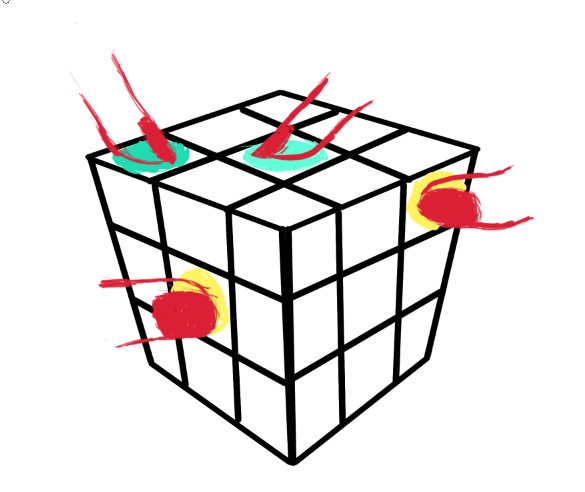
\includegraphics[width=18em]{pic1.png}\\
  \caption{}\label{1-1}
\end{minipage}
\begin{minipage}{0.5\linewidth}
  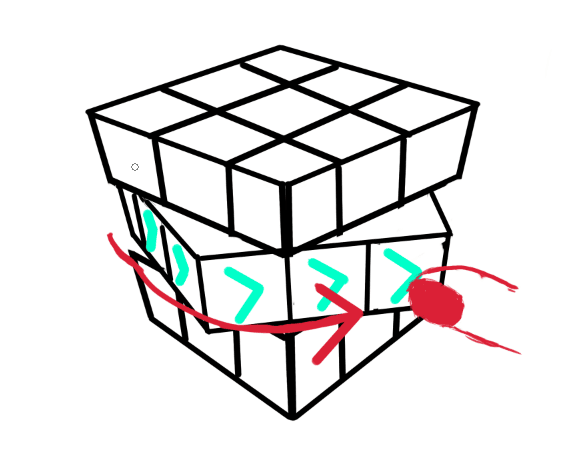
\includegraphics[width=18em]{pic2.png}\\
  \caption{}\label{1-2}
\end{minipage}
\end{figure}
\paragraph{}
本款产品作为一款音乐游戏,力图突破传统音游的游戏方式,使用最新的交互技术LeapMotion,给玩家提供最新潮的玩法。
\paragraph{}
由于LeapMotion的限制,Cubeat将是一款PC音乐游戏。
\newpage
\section{用户分析和需求}
\subsection{用户分析}
\paragraph{}
为了调查市场,我们组制作了一份调查问卷,主要针对青少年和大学生群体进行了调查。
\paragraph{对音乐游戏的熟悉程度}
\paragraph{}
我们首先针对大家对音乐游戏的了解程度做了调查
\begin{figure}[H]
  \centering
  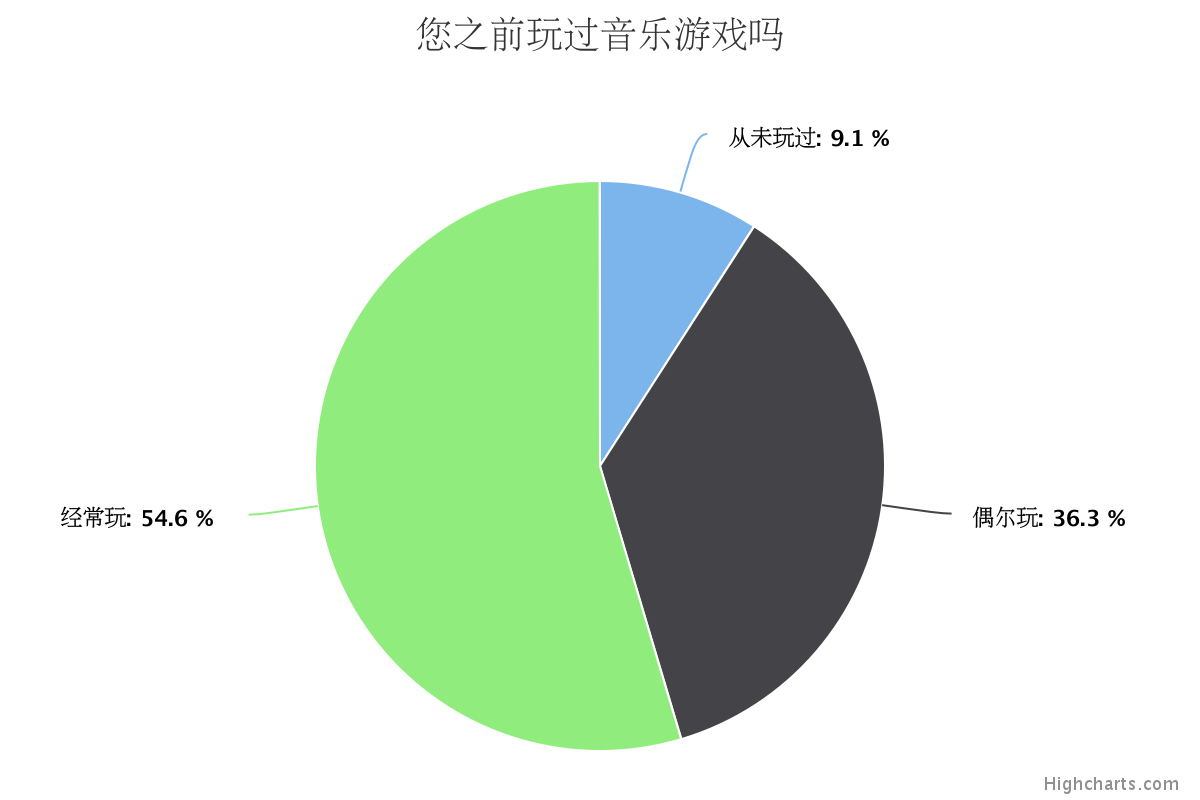
\includegraphics[width=22em]{chart1.png}\\
  \caption{您之前玩过音乐游戏吗}\label{2-1}
\end{figure}
\paragraph{}
由于在调查时,一些人表示不熟悉音乐游戏而拒绝了填写问卷,并且调查时间较短,所以推测数据有一定偏差。但从目前的数据来看,大多青少年和大学生都
玩过音乐游戏,一大半的人经常玩音乐游戏,可以看出音乐游戏的市场还是较为广阔。
\paragraph{玩音乐游戏的平台}
\begin{figure}[H]
  \centering
  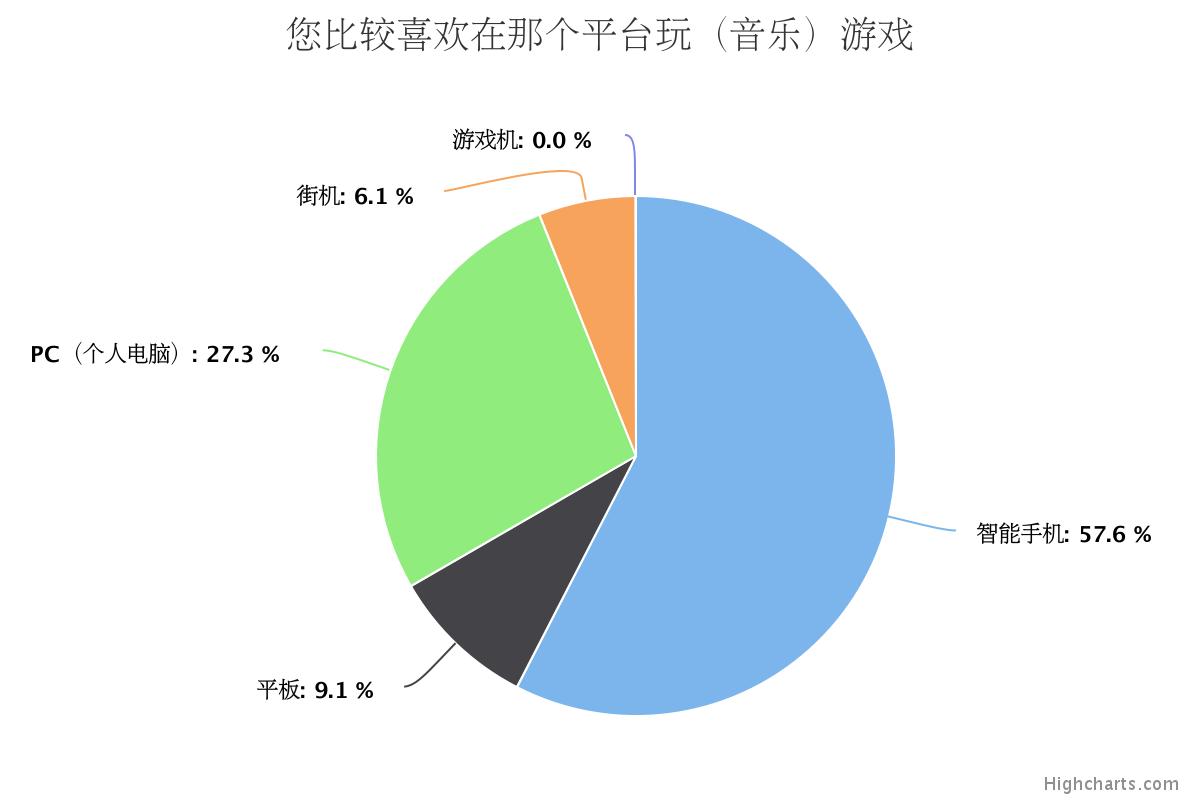
\includegraphics[width=22em]{chart2.png}\\
  \caption{您一般在那个平台玩(音乐)游戏}\label{2-2}
\end{figure}
\paragraph{}
随着智能手机的兴起,大家的娱乐时间日渐碎片化,从调查结果中也可见一斑。现在也有许多音乐游戏厂商在向智能手机或平板等移动设备进军,如:在日本火爆的LoveLive、腾讯的节奏大师、雷亚的deemo和在内测中的VOEZ。
但是不可否认的是PC端仍是许多玩家特别是精英玩家的必选平台,为音乐游戏,作为一种注重培养精英玩家的游戏,快餐式的游戏体验不能给玩家带来许多乐趣。因为音乐游戏需要快速反应和对音乐的熟悉来获取更好的成绩,
想要提高水准,一般只能用圈内所说的“堆PC”,也就是多次尝试来达成。而愿意花费大量时间的玩家往往不会在乎平台的区别,所以我们认为PC客户端的Cubeat在音游圈仍旧有不错的市场。
\paragraph{尝试新的操作方式?}
面对新鲜事物,大部分玩家选择乐于接受的态度
\begin{figure}[H]
  \begin{minipage}{0.5\linewidth}
  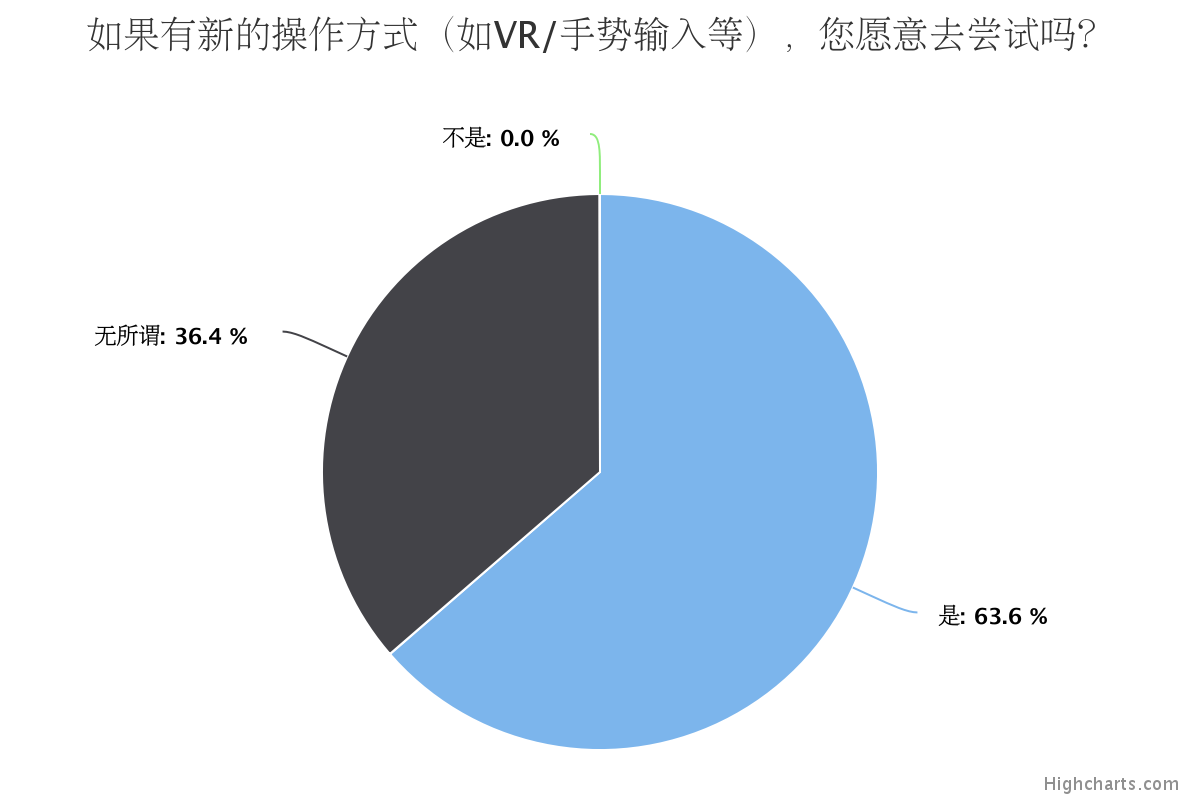
\includegraphics[width=20em]{chart3.png}\\
  \caption{}\label{2-3}
\end{minipage}
\begin{minipage}{0.5\linewidth}
  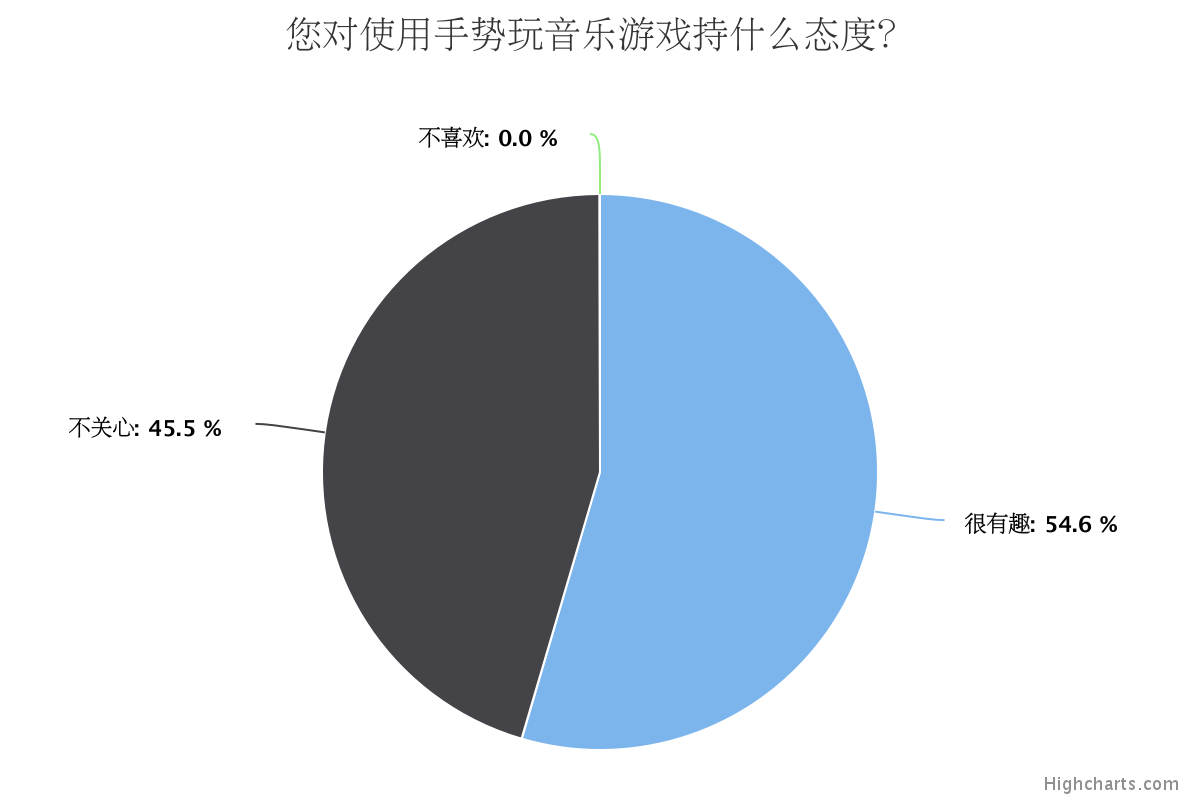
\includegraphics[width=20em]{chart4.png}\\
  \caption{}\label{2-4}
\end{minipage}
\end{figure}
\paragraph{}
游戏玩家对于新鲜的事物总是投以最高的好奇和憧憬,特别是新的与游戏的交互模式,相信吸引到不少用户的眼球。但是新的交互方式也意味着新的缺陷,现在手势输入还未普及,大部分玩家没有LeapMotion等设备,
这也将是我们推广的一个限制。但是最近游戏厂商占领VR市场之风越演越烈,Sony、Vavle纷纷加入竞争,大力推广VR设备,相信不久的将来,VR/AR游戏将会是游戏市场的一大发展方向,也会有更多的人进入VR的世界,进行游戏。
所以Cubeat也顺应了游戏市场的方向。
\paragraph{是否愿意尝试Cubeat类的游戏}
\paragraph{}
由于实际游戏效果很难用文字或者图片描述,所以本调查结果仅供参考
\begin{figure}[H]
  \centering
  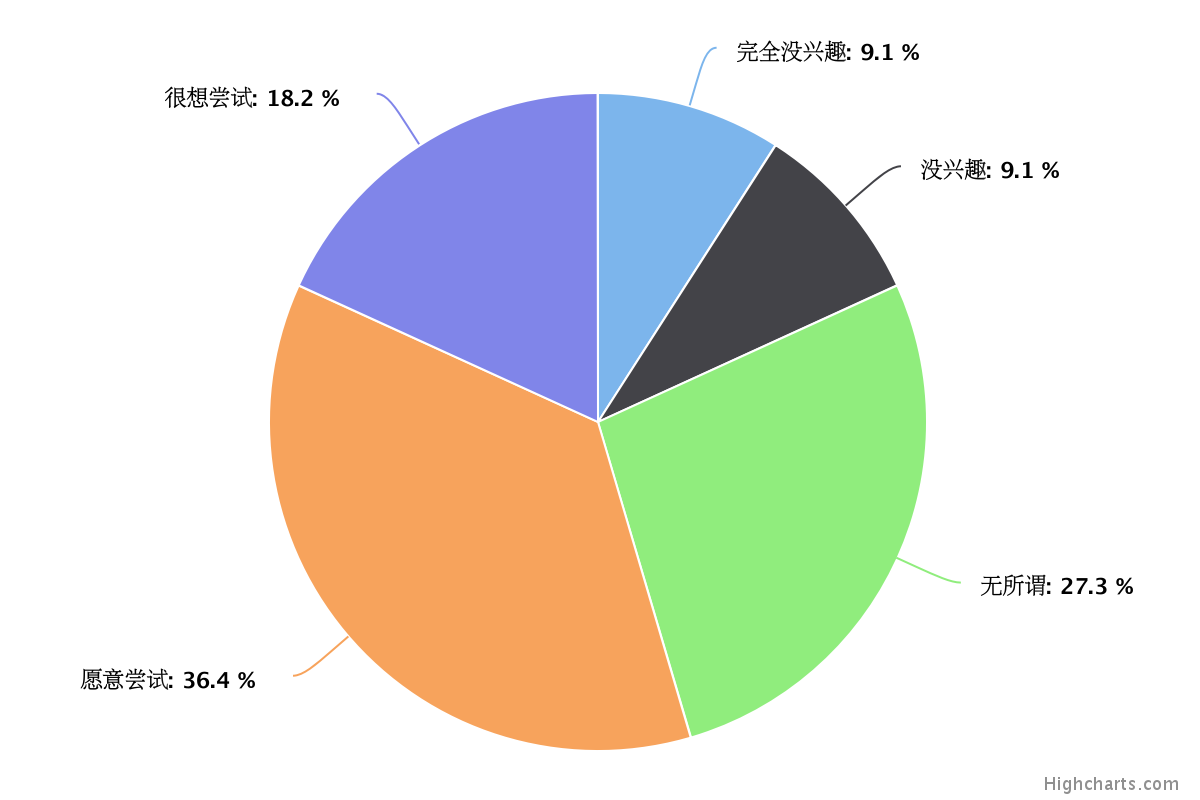
\includegraphics[width=22em]{chart5.png}\\
  \caption{是否愿意尝试以模仿作为载体手势输入的音乐游戏}\label{2-5}
\end{figure}
\paragraph{}
总之,调查结果出乎我们的意料。以往我们以为音乐游戏受众群体较小,但实际上年轻人中有许多人在玩音乐游戏。只是音乐游戏由于它自身的特性,很难获得精英玩家,导致许多玩家没有把主要精力放在音游上,而只是把它当做半个“音乐播放器”使用。
\paragraph{}
由于Cubeat输入方式的特性,我们游戏的可玩性将集中在玩法上,即使不愿意花费太多时间提高技术的玩家,也能从Cubeat中获得许多乐趣。
\subsection{同类产品}
\paragraph{}
分析完了用户,再从同类产品的角度分析一下Cubeat的可行性。在介绍同类产品之前,先介绍一下音游的几个基本概念
\begin{description}
  \item[谱面/难度] 在音乐游戏中,一首歌曲往往有多个难度,以供不同级别的玩家挑战。“谱面”或者“难度”一般就是指一首歌的某一个特定难度
  \item[note/物件] 一般指游戏中可供玩家击打的最小单位,一般对应音乐的一个音符或一个长音
  \item[BPM] beat per minutes 的缩写,乐曲的每分钟节拍数,用来衡量曲子的快慢。一般来说BPM越高的曲子,谱面越难
\end{description}
\paragraph{}
不同音乐游戏尽管画面不同,玩法不同,但是由于其以音乐为主体,总是逃不过这些概念和设计。
\paragraph{从“劲乐团”到“节奏大师”}
\paragraph{}
下落式(用按键或者触摸屏模拟弹钢琴)音乐游戏,作为音乐游戏的一大始祖,在PC还未流行时就已经在各大游戏机和街机上盛行。下落式非常精妙地设计了音乐游戏中音乐跟游戏连接的方式:使用钢琴键作为用户输入的接口,使用下落的音符作为音乐的接口。这种玩法一定程度上模拟了弹钢琴的动作,使得游戏简单直接容易让玩家上手。从十几年前的“劲乐团(O2jam)”到几年前的“节奏大师”、“deemo”等,均使用这个简单直观的设计,却都获得了很高的评价。
\begin{figure}[H]
\begin{minipage}{0.5\linewidth}
  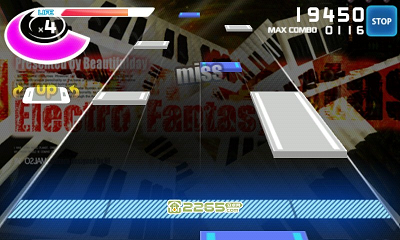
\includegraphics[width=15em]{O2jam.png}\\
  \caption{O2jam游戏截图}\label{3-1}
\end{minipage}
\begin{minipage}{0.5\linewidth}
  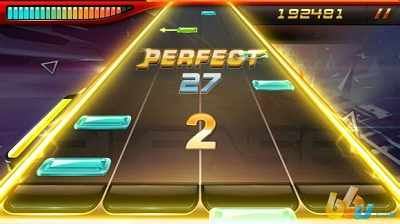
\includegraphics[width=15em]{rm.png}\\
  \caption{节奏大师游戏截图}\label{3-2}
\end{minipage}
\end{figure}
\paragraph{}
经历了十几年的发展,从最开始的玩家爆炸发展,到现在的审美疲劳,下落式音乐游戏已经渐渐走向衰落。从“劲乐团”到“节奏大师”,游戏模式没有变化,只是一个模子从PC被搬到了移动设备上来。
“劲乐团”早已关服停运,“节奏大师”玩家也不增反减,许多玩家抱怨下落式这种传统的游戏模式已经难以给自己带来乐趣。\\
\textbf{比较}
\begin{description}
  \item[玩法] 玩法陈旧缺乏创意,玩家慢慢审美疲劳
  \item[可玩性] 只有按键一种操作,较为单调
  \item[平台] 可以在PC/移动设备/街机上游戏,适用面较广
\end{description}
\paragraph{创新、变革}
音乐游戏是个大的话题,游戏制作者不会拘泥于一种玩法,许多标新立异的音乐游戏也是层出不穷。它们或是模拟除钢琴外其他乐器,或是用其他领域简单直观的东西代替琴键,成为玩家游戏的输入。下面举几个有代表性的这类作品
\paragraph{}
\textbf{乐动魔方}\\
乐动魔方是Konami公司出品的一款街机音乐游戏,后被移植到IOS和安卓平台。游戏方式十分简单,即在一个4X4的格子上会伴随音乐出现一些标示,玩家需要等待最佳时机点击标示,也就是音游圈俗称的“打地鼠”模式。
\begin{figure}[H]
  \centering
  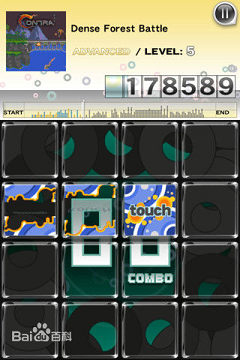
\includegraphics[width=20em]{gm1.png}\\
  \caption{乐动魔方}\label{3-3}
\end{figure}
\paragraph{}
乐动魔方要求玩家在16个格子上精准点击,比较难的谱面甚至会同时出现5、6个note需要玩家点击。所以玩家一般都在街机或是平板上玩“乐动魔方”。另外,虽然它脱离了下落式的束缚,但是相对简单的画面和玩法
也容易让玩家审美疲劳。但是作为Konami公司的产品,众多的原创音乐支持了它健康地发展,并在音游市场站稳了脚步。
\textbf{比较}
\begin{description}
  \item[玩法] 较传统音游有所进步,但是输入方式仍有限制,需要在较大的屏幕甚至游戏厅的街机上玩。Cubeat则只需带一个小巧的LeapMotion即可
  \item[内容] 官方提供乐曲和乐谱,玩家可以根据官方乐曲自制乐谱,内容有限。Cubeat支持玩家自己输入乐曲自制谱面
\end{description}
\newpage
\paragraph{}
\textbf{Lovelive!}\\
“Lovelive!”,大名鼎鼎的LL是音乐娱乐公司Lantis的一项大型企划中的音乐游戏,在多个平台有多个版本,这里主要介绍的是它在智能手机和平板上发售的版本。游戏本身玩法传承下落式,只不过用圆圈代替了方形的按键,并把水平的“钢琴”变为了一个半弧形。
\begin{figure}[H]
  \centering
  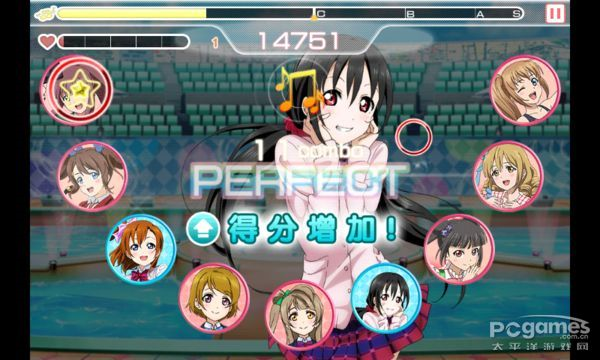
\includegraphics[width=24em]{ll.png}\\
  \caption{Lovelive!游戏画面}\label{3-4}
\end{figure}
\paragraph{}
Lovelive!作为较早将音乐游戏和手机游戏流行的“抽卡”、“活动”等元素结合起来的一款游戏,首先在日本获得了超高的人气。但是与其说它的成功是游戏模式,不如说它的成功
是整个企划的成功,是游戏人物和歌曲的成功。LL以动漫作为载体,用可爱漂亮的游戏人物,吸引了大量动漫爱好者的喜爱,LL粉丝众多,一些粉丝痴迷程度一度被称为“邪教”。所以对于二次元不感冒的人来讲,
LL可能只是个相貌平平的普通手机游戏
\paragraph{}
另一方面,LL作为一款网络手机游戏,继承了一般手机游戏吸引玩家和增加玩家投入时间的方式。高频率的活动,和需要很高的时间精力甚至财力的投入才能获取的活动回报,从某种程度上来讲不是一种很健康的游戏模式\\
\textbf{比较}
\begin{description}
  \item[玩法] 实质上仍旧是下落式,没有什么突破。但是学习了手机游戏的套路,增加了玩家游戏时间。Cubeat在玩法上创新,它的地图编辑器也可以为玩家提供额外的乐趣
  \item[设定] 与其他音乐游戏不同,Lovelive!拥有完整的人物背景故事设定,丰富的人物和剧情为游戏增加了许多分数。Cubeat不以设定作为最大卖点,这也是众多音乐游戏的选择
  \item[画面] 主要使用了动漫风格的画面和人物,Cubeat则将使用简洁干净的扁平化风格,让画面显得更加炫酷和前卫
\end{description}
\paragraph{立体输入的Cubeat}
音乐游戏在发展的过程中,不同厂商一直在尝试使用各种办法创新游戏模式,使玩家获得更新的游戏体验。虽然许多不经常玩音乐游戏的用户觉得与真实演奏场景或者太过抽象的操作方式,会使得游戏变得难以操作。
但事实证明只要设计合理,“模拟乐器”就只是个做音乐游戏的最“navie”的想法。无数音乐游戏探索的道路中,也许更具有立体感的手势输入就是其中之一吧。也许街机游戏也能做到类似的想过,但是它可不能像LeapMotion一样随身携带
\subsection{需求分析总结}
\paragraph{}
总的来说,音乐游戏作为游戏业不小的一个分支,体验玩家不少,但缺少精英玩家,仍旧有较大的市场潜力。而音乐游戏在经过了数十年平稳的发展后,正在和网络、移动端、VR等新时期的元素融合。不同音乐游戏的侧重点也不尽相同。
Cubeat正式应用了手势输入这个新元素的一款新时期的音游。很多玩家也很希望尝试新鲜的游戏方式,所以会很乐于尝试这款游戏。
但是硬件设备仍旧是遏制新元素发展的关键因素:许多用户没有LeapMotion等设备,LeapMotion较高的价格......都给我们的推广带来了不小的挑战
\paragraph{}
好在当今行业发展迅猛,网络也为我们提供了广阔的渠道。我们可以在一些平台(如LeapMotion App Store)上积累人气,相信相关硬件也会迅速发展。等待技术真正发展普及手势输入,我们的游戏可以做得更好。
\begin{figure}[H]
  \centering
  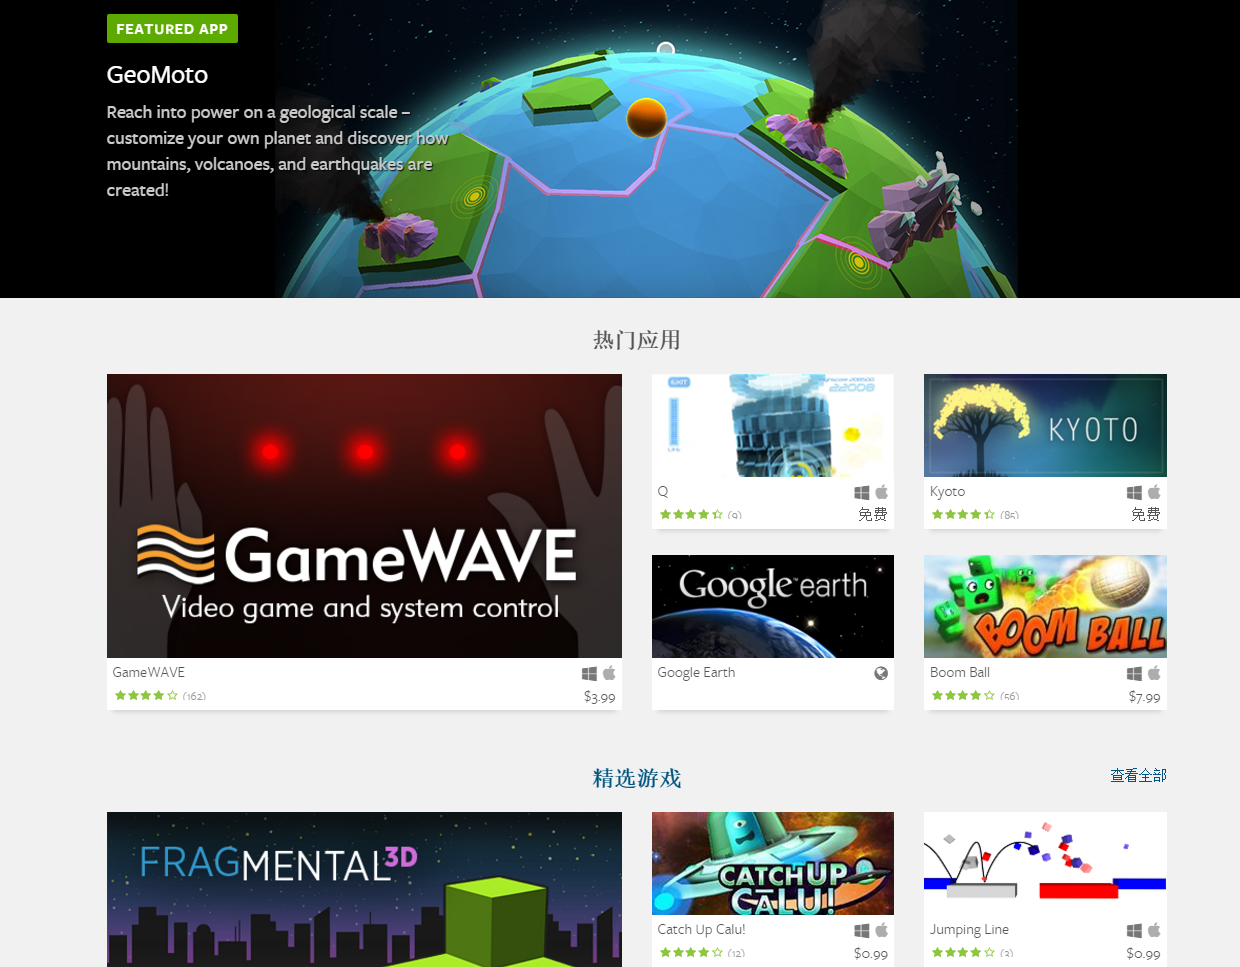
\includegraphics[width=24em]{leapMotionAppStore.png}\\
  \caption{LeapMotion App Store截图}\label{3-5}
\end{figure}
\newpage
\section{目标}
做出有一定游戏性的通过识别手势进行输入的一个音乐游戏。作为一款音乐游戏,应该具有以下特性:
\begin{description}
  \item[完善的UI界面] 为用户提供基本的图形界面交互
  \item[丰富炫酷的游戏画面] 有一定的画面特效,用炫酷的画面给玩家更多积极的反馈
  \item[完整的游戏模式] 以音乐为背景,使玩家的操作需要契合节拍
\end{description}
\paragraph{}
除此之外,我们还有以下较其他音乐游戏创新的功能
\begin{itemize}
  \item 自带编辑器功能,让玩家也能轻松参与到编谱中来,方便构成玩家社区
  \item 多种基本手势输入法,比如手指点击,滑动,手掌翻动等
  \item 优化LeapMotion的手势输入识别,让玩家更畅快地玩Cubeat
\end{itemize}
\paragraph{}
基础玩法现在设计有两种,即有两种note:用手指戳击魔方的某一个方块,用手指拨动魔方的某一层。
\begin{figure}[H]
  \centering
  % Requires \usepackage{graphicx}
  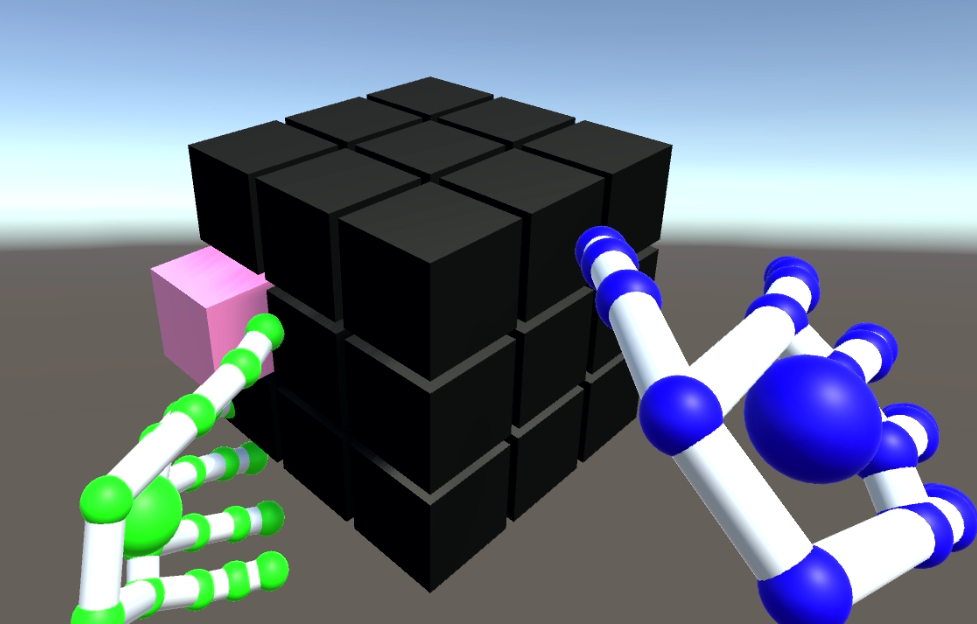
\includegraphics[width=24em]{demo.png}\\
  \caption{demo效果图}\label{4-1}
\end{figure}

\section{创新点}
\subsection{手势输入}
\paragraph{}
\textbf{应用最新的LeapMotion作为手势输入支持}
LeapMotion(中文名:厉动),于2013年2月27日发布。它是一款面向PC和Mac的体感控制器,可以捕捉人类的手部动作。
经历了三年的成长,它的硬件和软件系统都有了长足的提升。它使用红外线摄像头以超高频率捕捉用户的手部特征,能够准确识别出人体手部的数十个关节,并重绘其三维位置
\begin{figure}[H]
\begin{minipage}{0.5\linewidth}
  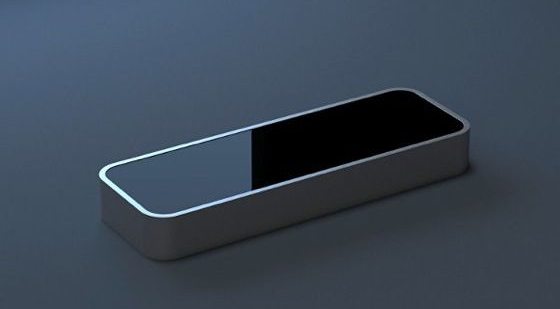
\includegraphics[width=15em]{leap.png}\\
  \caption{LeapMotion实物图}\label{3-1}
\end{minipage}
\begin{minipage}{0.5\linewidth}
  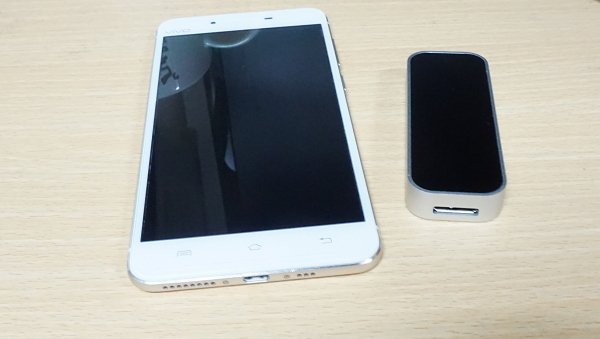
\includegraphics[width=15em]{leapCompare.png}\\
  \caption{LeapMotion大小比对}\label{3-2}
\end{minipage}
\end{figure}
\paragraph{}
LeapMotion本体大小只有$7.8\times2.8\times1.1$,远远比一般的智能手机要小。现在中国售价在400-500元
\paragraph{}
使用LeapMotion,实现了我们与其他音乐游戏最大的不同点——手势输入,让玩家脱离键盘、屏幕或是街机的束缚,用双手自由享受音乐游戏的乐趣
\paragraph{}
当然,如何让用户玩起来“爽”也是一个艰难的课题。我们前期做了一个demo,感觉LeapMotion精度尚可,只是由于时间紧迫,没有完全实现玩法设计,也没有配合上音乐,没有实质性体验。
我们将不断调整优化玩法,使得Cubeat的操作更加流畅、体验更加出色。
\subsection{玩家可编辑图谱}
\paragraph{}
开源社区是慢慢流行起来的一种代码管理开发方式,音乐游戏也能做到开源的效果。Cubeat将为玩家提供一个谱面编辑器,能让玩家用自己想用的歌曲随意进行谱面的制作。
将来如果开发网络支持,提供谱面上传和排行功能,将为游戏提供无穷的可能,也可以建立去一个可发展的游戏社区,游戏社区也将反向支持更多玩家和精英玩家的出现。
\newpage
\section{技术支持和分工}
\subsection{技术}
\paragraph{}
\textbf{深入了解Leap Motion SDK}
这个技术需求是针对游戏的操作体验的。仅仅使用Leap Motion预定义的操作样本无法满足我们的体验需求。在我们尝试过之前的简单demo之后我们发现了几个缺陷。一是手指会穿透魔方,这个给人感觉非常不自然。二是手指的动作略显僵硬。针对这两个缺陷我们需要在Leap Motion的基础上开发适合这个魔方音游的手势操作接口。首先要设计并实现手指不会穿透魔方并且看上去自然的手部操作映射,其次可以做指尖动作的局部放大功能。
\paragraph{}
\textbf{音乐游戏的判定机制和编辑器的相关技术}
这个技术需求是针对游戏机制的。音乐游戏在判定上较为严格并且有不同level的打击判定。长音符和短音符在操作和打击判定上也有比较大的区别。如何设计实现适合Cubeat的打击判定机制也是一个技术难点。在编辑器方面,由于编辑谱面需要时间轴,操作判定节点、音乐三者结合,并且我们没有相关编辑器的开发经验,因此这个编辑器的实现有较大的技术风险。
\paragraph{}
\textbf{音乐游戏的特效}
这个技术需求是针对游戏视觉反馈的。音乐游戏玩起来是否让人感觉爽在很大程度上取决于它的视觉反馈。不同level的打击有不同强度的反馈。由于我们在操作上缺少了触觉载体,因此视觉反馈尤为重要,打击特效的设计和制作需要运用三维设计软件和图形学中的一些特效技术。在实现打击特效的基础上进阶还可以给游戏加上整体的随着音乐律动的背景效果。
\subsection{分工}
\paragraph{}
\textbf{杨 铭 5130379022}
主要负责Leap Motion的深入学习和对其手势操作进行调整以及整合游戏机制、手势控制和界面特效。
\paragraph{}
\textbf{李 晟 5130379017}
主要负责游戏特效,ui界面的设计实现。
\paragraph{}
\textbf{张云翔 5130379012}
主要负责游戏机制和编辑器的设计实现。
\paragraph{}
以上的分工会根据工作量和成员能力的不同做一定的调整。
\end{document}
